\chapter{Pithos Design}
\label{chp:DESIGN}

The generic state consistency model was presented in Section \ref{generic_event_update_model}, but one of the key challenges that still remain was determined to be the design of an authoritative storage module specifically tailored to P2P MMVEs. The authoritative storage module identified in the generic consistency model state management and state persistency for the authoritative objects.

In the previous chapter, we've identified the main requirements of P2P MMVE state management and persistency as: fairness, overhead, reliability, responsiveness, scalability and security. It is argued that none of the current approaches to state persistency satisfy all identified requirements. This chapter proposes a novel design, called Pithos, that satisfies all the identified requirements for P2P MMVEs.

The novelty of Pithos lies in its group-based distance-based approach that supports both a responsive and a fair storage system, while also taking into account security aspects of scalable distributed storage. There are some storage systems that provide responsive or fair storage, but none that provide both. No storage system, designed specifically for P2P MMVEs, have taken security into account.

If Pithos is incorporated into an existing P2P MMVE consistency architecture, it will add the ability to robustly handle both state management and state persistency. The addition of a robust state management and persistency mechanism, specifically designed for P2P MMVEs, will bring us one step closer to the creation of a complete P2P MMVE architecture.
%%%%%%%%%%%%%%%%%%%%%%%%%%%%%%%%%%%%%%%%%%%%%%%%%%%%%%%%%%%%%%%%%%%%%%%

\section{Use cases}
\label{use_cases_goals}

The purpose of Pithos is to allow for efficient object storage and retrieval that satisfies all identified requirements. As is evident from authoritative storage in the flow diagram in Figure \ref{fig_event_update_flowdiagram}, Pithos will interface directly with the VE logic, as well as receive updates from the update generator. For the purposes of this discussion, update generation is assumed to be part of VE logic.

\begin{figure}[htbp]
 \centering
 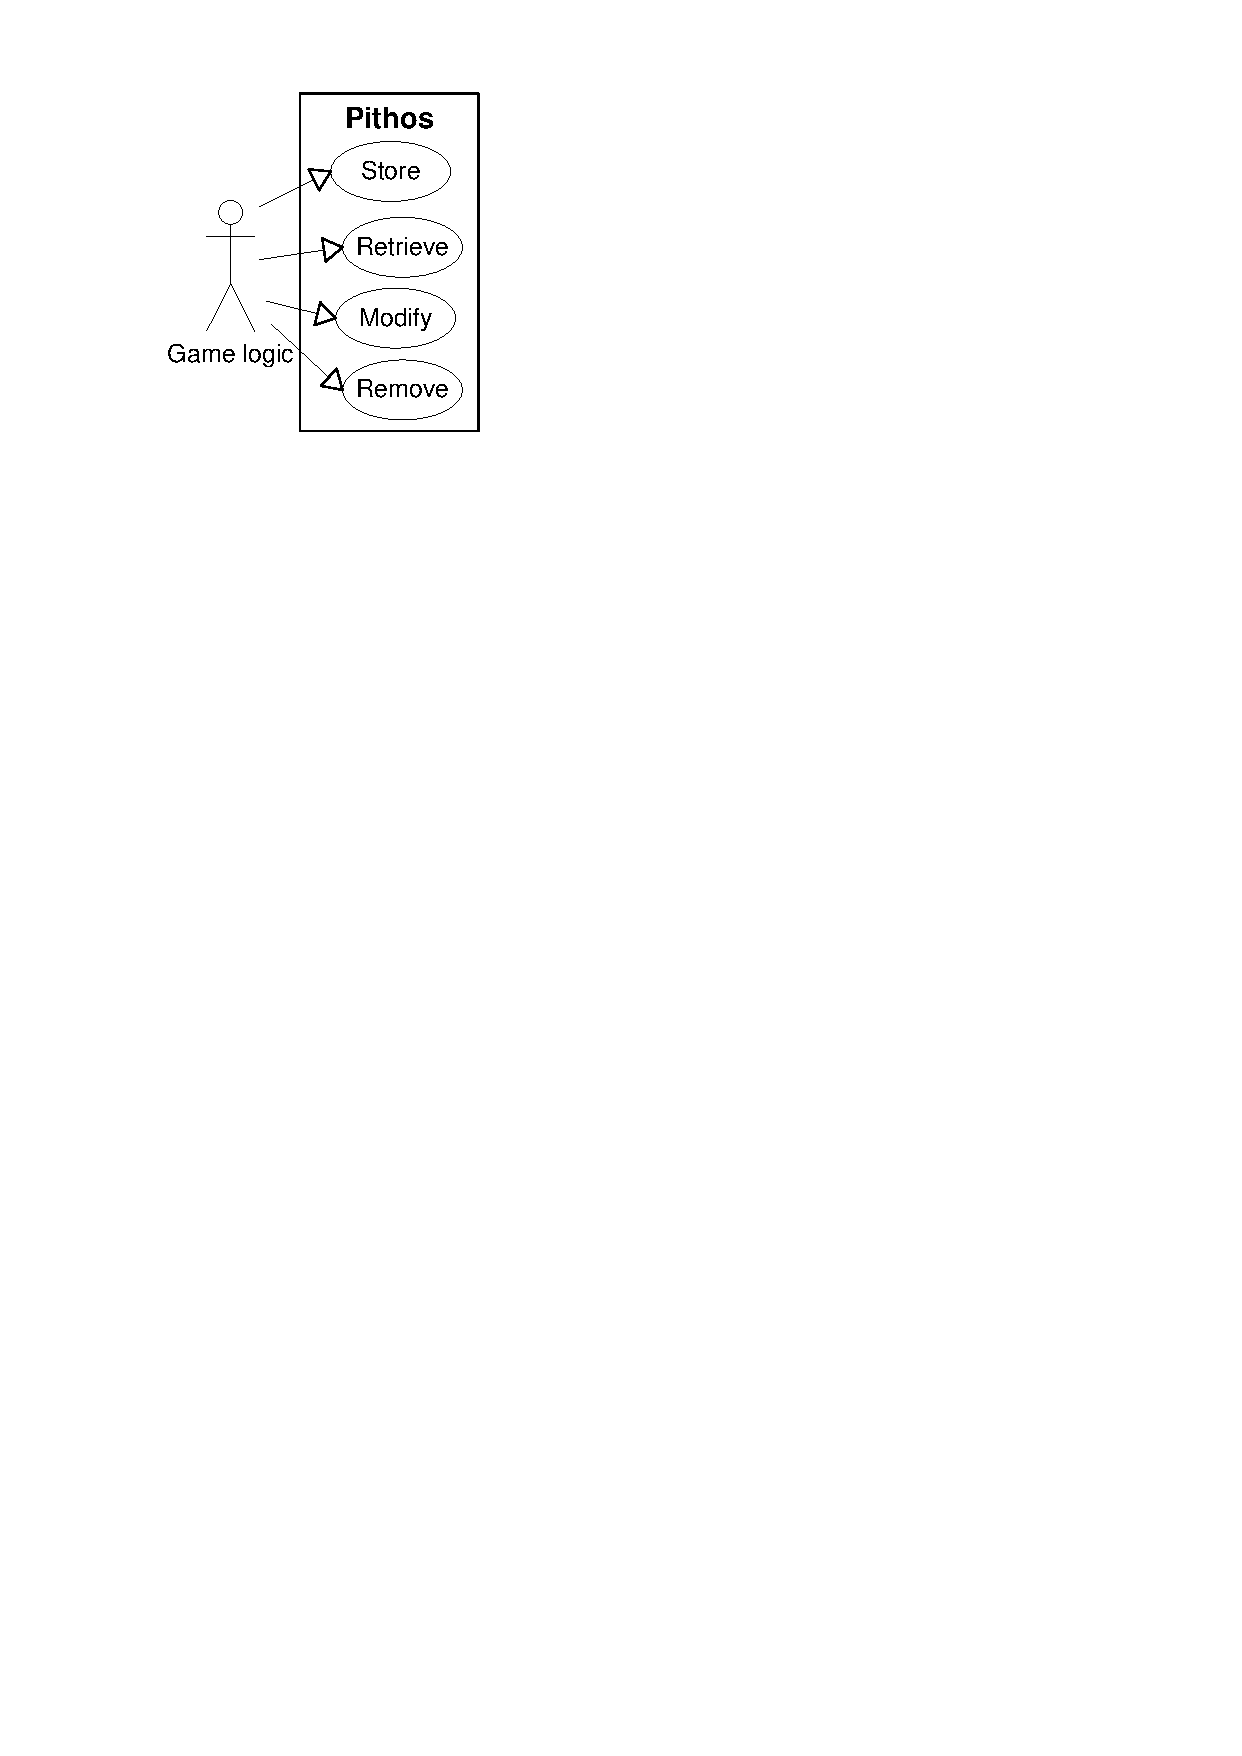
\includegraphics[clip=true, viewport=28mm 223mm 82mm 282mm, width=0.3\textwidth]{pithos_use_case}
 \caption{Use case diagram of Pithos}
 \label{fig_pithos_use_case}
\end{figure}

As shown in the use case diagram in Figure \ref{fig_pithos_use_case}, the VE logic should be able to use Pithos in four ways: store, retrieve, modify and remove. These are the use cases generally required of any storage system.

\subsection{Store}

The VE logic will store data when a new object is added to the VE state. This can happen as a consequence of an event leading to the generation of a new object. An example of this is a rocket firing at a target. This event might generate a missile object to be sent towards the target.

\subsection{Retrieve}
Object retrieval will be required every time an event is received. The VE logic will retrieve the object state from memory, which is part of state management. Object states, other than the one being altered, might also be required by the logic to determine the effect an event will have, as discussed in Section \ref{event_logic_update}.

\subsection{Modify}
Object modification occurs every time an object update is generated. An object update, by definition, required a modification of the object state.

\subsection{Remove}
Object removal might also be required to save storage space, although this is not essential to the correct functioning of the storage system.

\section{Designing for the storage requirements}

Pithos is designed to fulfill all use case requirements as well as the storage requirements for P2P MMVE storage architectures as set out in Section \ref{key_challenges_cm}. To achieve both these goals, an architecture was first designed to fulfill all the storage requirements and the use case requirements were then implemented on the designed network.

The inspiration for Pithos come from two observations:
%
\begin{enumerate}
  \item One can combine multiple storage models and arrive at a model which possesses fewer disadvantages than any of the models used.
  \item Responsiveness is greatly increased in a fully distributed model, where there is no intermediate server that relays all information.
\end{enumerate}

Fully distributed architectures are, however, not scalable because the number of messages scaling by $O(N^2)$, where $N$ is the number of nodes in the network. We, therefore, use groups of peers, where all the peers in a group are fully connected.

This section will describe how the design of Pithos satisfies the identified storage requirements. For each of the requirements of fairness, reliability, responsiveness, scalability and security, the design decisions made to achieve the specific requirement will be discussed. Some design decisions satisfy multiple requirements, therefore different requirements might discuss the same design decision, with a focus on how the decision satisfies the specific requirement.

\subsection{Responsiveness}

In Pithos, responsiveness is achieved by grouping users into fully connected groups, using group-based distance-based storage to distribute objects and using replication to enable the parallel retrieval of objects.

\subsubsection{Group storage}

In a fully connected network, where all nodes are connected to all other nodes, every node is one hop away from every other node. This solution is, however not scalable. In order to achieve a scalable single hop architecture, it was decided to group users in the virtual world. User groups are then fully connected, which allows for highly responsive group interactions. Group sizes are smaller than the overall network size and allows for the fully connected groups to remain scalable.

In virtual worlds, users already group themselves into explicit groups, including questing groups, raid groups and guilds. In Section 3.1 of \cite{varvello_phd}, it was found that most users in Second Life form small groups.  Implicit groups are also formed by flocking, where multiple users congregate in areas of the virtual environment that are of interest to them \cite{flocking}.

\subsubsection{Distance-based storage}
Grouping users is not sufficient to achieve a responsive system. Users should also require data stored in the group more than data stored outside the group. To this end, distance based storage is used on a group level. This means that objects are stored in the group that is closest to them. The assumption is that users interact more with objects that are closer to them and, therefore, have more interest in closer objects. If a user has interest in a far off object, she will likely move closer to that object.

\subsubsection{Replication}

Replication improves retrieval responsiveness, if multiple copies of an object may be requested in parallel and the object that arrives fastest is used. This is termed parallel retrieval in the Pithos design and is evaluated in Chapter \ref{chp:EVALUATION}.

Depending on how storage is implemented, replication can also improve storage responsiveness if the first object that is successfully stored signals success to the higher layer. This is termed ``fast storage'' in the Pithos design, the suitability of which is evaluated in Chapter \ref{chp:EVALUATION}.

\subsection{Reliability}

Reliability is achieved by storing all objects on overlay storage (DHT), in addition to group storage, replicating all stored objects and repairing object replicas as they are removed due to network churn.

\subsubsection{Overlay storage}
Distance-based group storage attempts to maximize the number of requests for objects within a group. The number of actual intra-group vs. inter-group requests will still depend on the grouping algorithm and it might not be possible to ensure that all requests remain in the group.

In order for peers to be able to requests objects stored in other groups, overlay storage is used. Peers belong to both a group and the overlay. Peers can therefore request data from the group and from the overlay. Overlay storage adds reliability by ensuring that out-of-group object request can also be served.

Every retrieve request is requested from both the group and the overlay storage. If any of the storage types fail, the other might still succeed, improving reliability.

\subsubsection{Replication}

Replication allows for multiple peers to leave the network before an object becomes unavailable, improving reliability. Because of network churn, replication is essential to ensuring objects survive network churn. If only a single object is stored, a node unexpectedly leaving the network destroys an object. There is no chance of an object being recovered if no replicas are used.

It is, therefore, important that a sufficiently large number of replicas and repair rate be chosen, while taking the network parameters such as expected node lifetime and required TTL into account. The interaction between these parameters are explored in Chapter \ref{chp:MODELLING}.

\subsubsection{Repair}

Repair further improves reliability by maintaining sufficient object replicas. When it is discovered that a peer has left the network, peers storing the objects of the peer that left can replicate those objects, thereby maintaining a sufficient number of replicas.

If only replication is used, the number of replicas will steadily decline from the moment the object is stored. A repair mechanism is needed to replace missing replicas, ensuring long term object survivability.

\subsection{Security}

Security cannot exist in a single system layer and has to be ensured on multiple layers, as discussed in Section \ref{characteristics_security}. Some security concepts implemented in Pithos are the use of a certification authority, replication and the use of quorum mechanisms.

\subsubsection{Certification}

A difference between Pithos and other P2P systems is that it requires all peers to be uniquely identifiable. A main requirement of classic P2P storage architectures is that peers remain anonymous to ensure user privacy. In Pithos, all users are unique identifiable. An object records which user created it and which users modified it. This allows for the identification of users that maliciously alter objects.

\subsubsection{Replication}

Storing multiple replicas attempts to limit the effect that a malicious user might have on the storage system. If a malicious user alters an object, the original unaltered object is still stored on multiple peers.

\subsubsection{Quorum}

When security is a concern, multiple parallel retrieval requests can be performed. A quorum mechanism is then used at the receiving peer to compare the different received objects. The object that is returned by most of the peers is then considered to be the correct object. A peer modifying an object has no effect on the system, since the receiving peer selects the object returned by the other peers.

The quorum mechanism will fail if the majority of peers queried colludes to send the same altered object. This can be detected by comparing received objects to objects received from the overlay storage. Ideally, it should only be necessary to perform this comparison if it is suspected that some of the peers in the group are colluding to maliciously alter objects.

\subsection{Fairness}

Fairness is achieved by using both overlay storage and group storage. Both of these schemes require all objects in the network to participate in storage.

\subsubsection{Group storage}

Objects are uniformly distributed on group peers, ensuring that all group peers share the load of group objects stored.

\subsubsection{Overlay storage}

Overlay storage maps objects and peers to the same uniform key space and stores an object on a peer that is the closest match for the object's key. This uniformly random mapping ensures a uniform distribution of objects in the overlay.

\section{Key modules and mechanisms}
\label{key_modules_mechs}

In this section we identify and discuss the key modules and mechanisms that Pithos requires to implement in order to achieve its design requirements.

\begin{figure}[htbp]
 \centering
 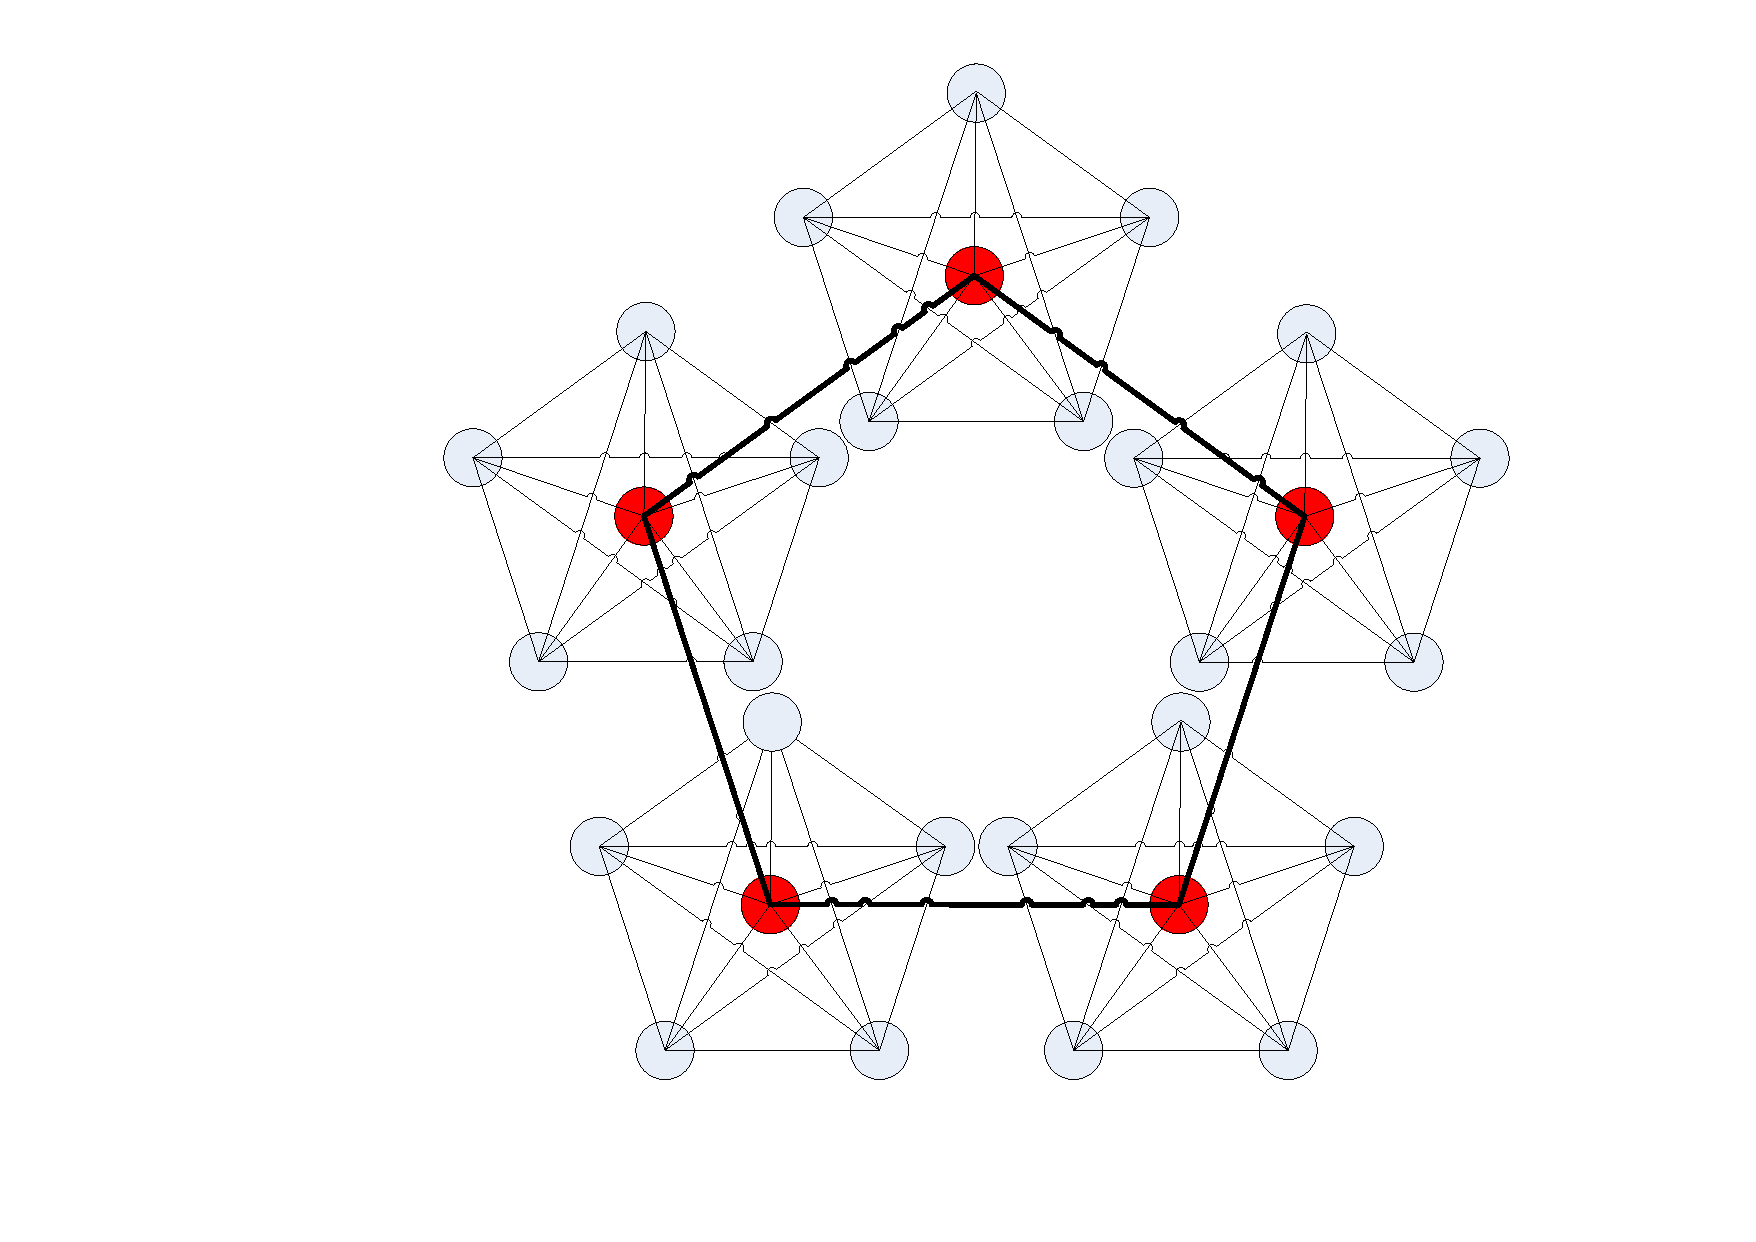
\includegraphics[clip=true, viewport=65mm 4mm 267mm 205mm, width=0.7\columnwidth]{CDHT_layout}
 \caption{Layout of the Pithos storage architecture}
 \label{fig_pithos}
\end{figure}
%
Figure \ref{fig_pithos} shows the Pithos network topology. The figure shows groups of fully connected peers (light blue) and super peers (dark red). All peers are further connected to a single overlay. Pithos groups peers to form a two tiered storage model. The first tier is a storage model at group level (group storage) and the second is a storage model over all groups (overlay storage). Pithos can be considered as a multi-tiered structured overlay, with group storage an implementation of an $O(1)$ overlay and overlay storage an implementation of an $O(\log (N))$ overlay.

When referring to state management and persistency as defined in Section \ref{management_persistency_def}, Pithos is designed to serve both requirements. Group storage is designed for state management and overlay storage for state persistency. Since state persistency does not require responsive storage, the overlay section of Pithos is well suited to this task, while group storage, with its high responsiveness is well suited to state management.

\subsection{Group storage module}

On a network level, group storage consists out of two node types: super peers and peers. It is possible for a single Pithos terminal to be both a peer and a super peer.

Since group storage can be seen as an $O(1)$ structured overlay, it requires the features identified in Section \ref{structured_overlay_features}: network topology, routing, network join and leave and bootstrapping. Additionally to the required routing features, group migration should also be possible (moving from one group to another) and records of all objects stored and all peers present are also required. Lastly, some method of determining group membership is required.

\subsubsection{Network topology and routing}

The network topology is fully connected and routing in such a network topology is trivial. A peer's routing table contains a list of all peers in the group. To route a message to a destination peer, the peer address is retrieved from the routing table and a message is sent directly to that peer.

\subsubsection{Super peers and peers}

In group storage, peers handle requests from the higher application layers. Peers also represent users in group storage, which means that peers are the originators of all store, retrieve, modify and remove requests from a group perspective. The peers themselves receive those requests from the higher layer (such as a game client).

%Super peer selection
Super peers are responsible for representing a group, managing group membership and managing object repair. The design of Pithos attempted to minimise super peer load, to prevent the functionality of the super peer to adversely affect the peer. The super peer does, however, require extra resources from the underlying system. It would, therefore, be preferable to select peers that have sufficient additional resources to become super peers.

The question of super peer selection has not yet received sufficient research attention. The authors in \cite{Suesselbeck_super_peer_selection} discuss the need for a utility function that is able to calculate the appropriateness of a peer to become a super peer. The utility function takes certain system parameters into account. The issue is that many of the identified parameters cannot currently be reliably measured, including for example: user reputation, bandwidth and delay. The super peer selection problem is, therefore, still an open research problem.

For the current Pithos design, it is assumed that some utility function exists to select the most appropriate peer and to promote that peer to super peer status.

\subsubsection{Join and bootstrapping mechanisms}
\label{join_mechanism_design}

Peers should be able to join the P2P network and join a group in the P2P network. The Pithos design specifies that some well known entry point into the P2P network should exist that a peer can use for bootstrapping. For an MMVE, it is recommended that this be a peer or a set of peers that is controlled by the VE operator. It is understood that this design breaks away from a pure P2P design, but a pure P2P design is not always the best design in practice.

It is assumed that VE operators want to control access to the VE. The operator controlled bootstrapping mechanism will aid in that goal. If the bootstrapping mechanism is fully distributed, operators might have no way to control access to their VEs, which would simplify the task of pirating the VE and creating a separate free VE.

A well known entry point into the network also simplifies the network design.

For a peer to join a group, it is assumed that some distributed grouping mechanism would exist. Super peer might form part of their own virtual location aware overlay network. A joining peer can then be passed from super peer to neighbouring super peer, until an appropriate peer accepts the peer's join request.

Peer joining will also depend on the specific grouping algorithm used.

\subsubsection{Grouping mechanism}
\label{grouping_design}

In order for Pithos to build groups, a clustering mechanism is required. There already exists a wealth of clustering algorithms in literature and a few will be reviewed here.

\emph{Distributed peer clustering techniques}: use the distance between users in the virtual environment to dynamically group users. The main idea of flocking is that users move around in groups, rather than randomly on their own. It is desirable that user density within groups should remain constant, because a fully distributed architecture is not scalable. This means that groups should merge or split as the user density within them change. It might also be required to have mobile groups, where a group has a velocity as well as a position, to be able to uniquely identify groups, even with users joining and leaving and the group moving through the virtual world.

Affinity propagation clusters nodes using a similarity matrix to find similar nodes \cite{affinity_propagation}. The similarity matrix may contain user positions. In this case, affinity propagation will group nodes depending on their location in a virtual world. This algorithm might be well suited to P2P applications, since it is a distributed clustering algorithm based on message passing.

\emph{Dynamic Voronoi regioning}: divides the virtual world into regions that can be resized or further divided to maintain constant user densities across regions. VSO \cite{VSO_Hu_Chen}, \cite{self_organising_sps_post} creates dynamic regions based on a Voronoi overlay network \cite{voronoi_diagrams_survey}. Near constant user density is achieved by increasing and decreasing the area sizes. This system is based on VON, a distributed Voronoi overlay network designed for MMVEs \cite{VON_VAST}.

Clustering is also used in mobile ad-hoc networks (MANETs) for routing purposes. Mobile-aware clustering algorithms used in MANETs, might also be applicable to P2P MMVEs \cite{clustering_survey}. Mobile-aware clustering uses relative velocities of mobile nodes to define clusters containing nodes with low relative velocity to each other.

Any of the above mentioned techniques might be used to achieve distributed clustering in P2P MMVEs. The focus of this work is, however, not on developing a novel clustering algorithm for P2P MMVEs, therefore we have chosen to use a super peer centered distance-based grouping approach for group clustering in our implementation. The implemented joining and grouping algorithms will be discussed in more detail in Section \ref{joining_and_grouping_imp}.

\subsubsection{Leave mechanism}
\label{leave_design}

If a peer leaves the network unexpectedly, it will not have the opportunity to inform its group. With no mechanism to detect a peer unexpectedly leaving, group inconsistency will occur. The peer that left might be selected to store an object or might be required to provide an object from storage. These requests will all fail.

\begin{figure}[htbp]
 \centering
 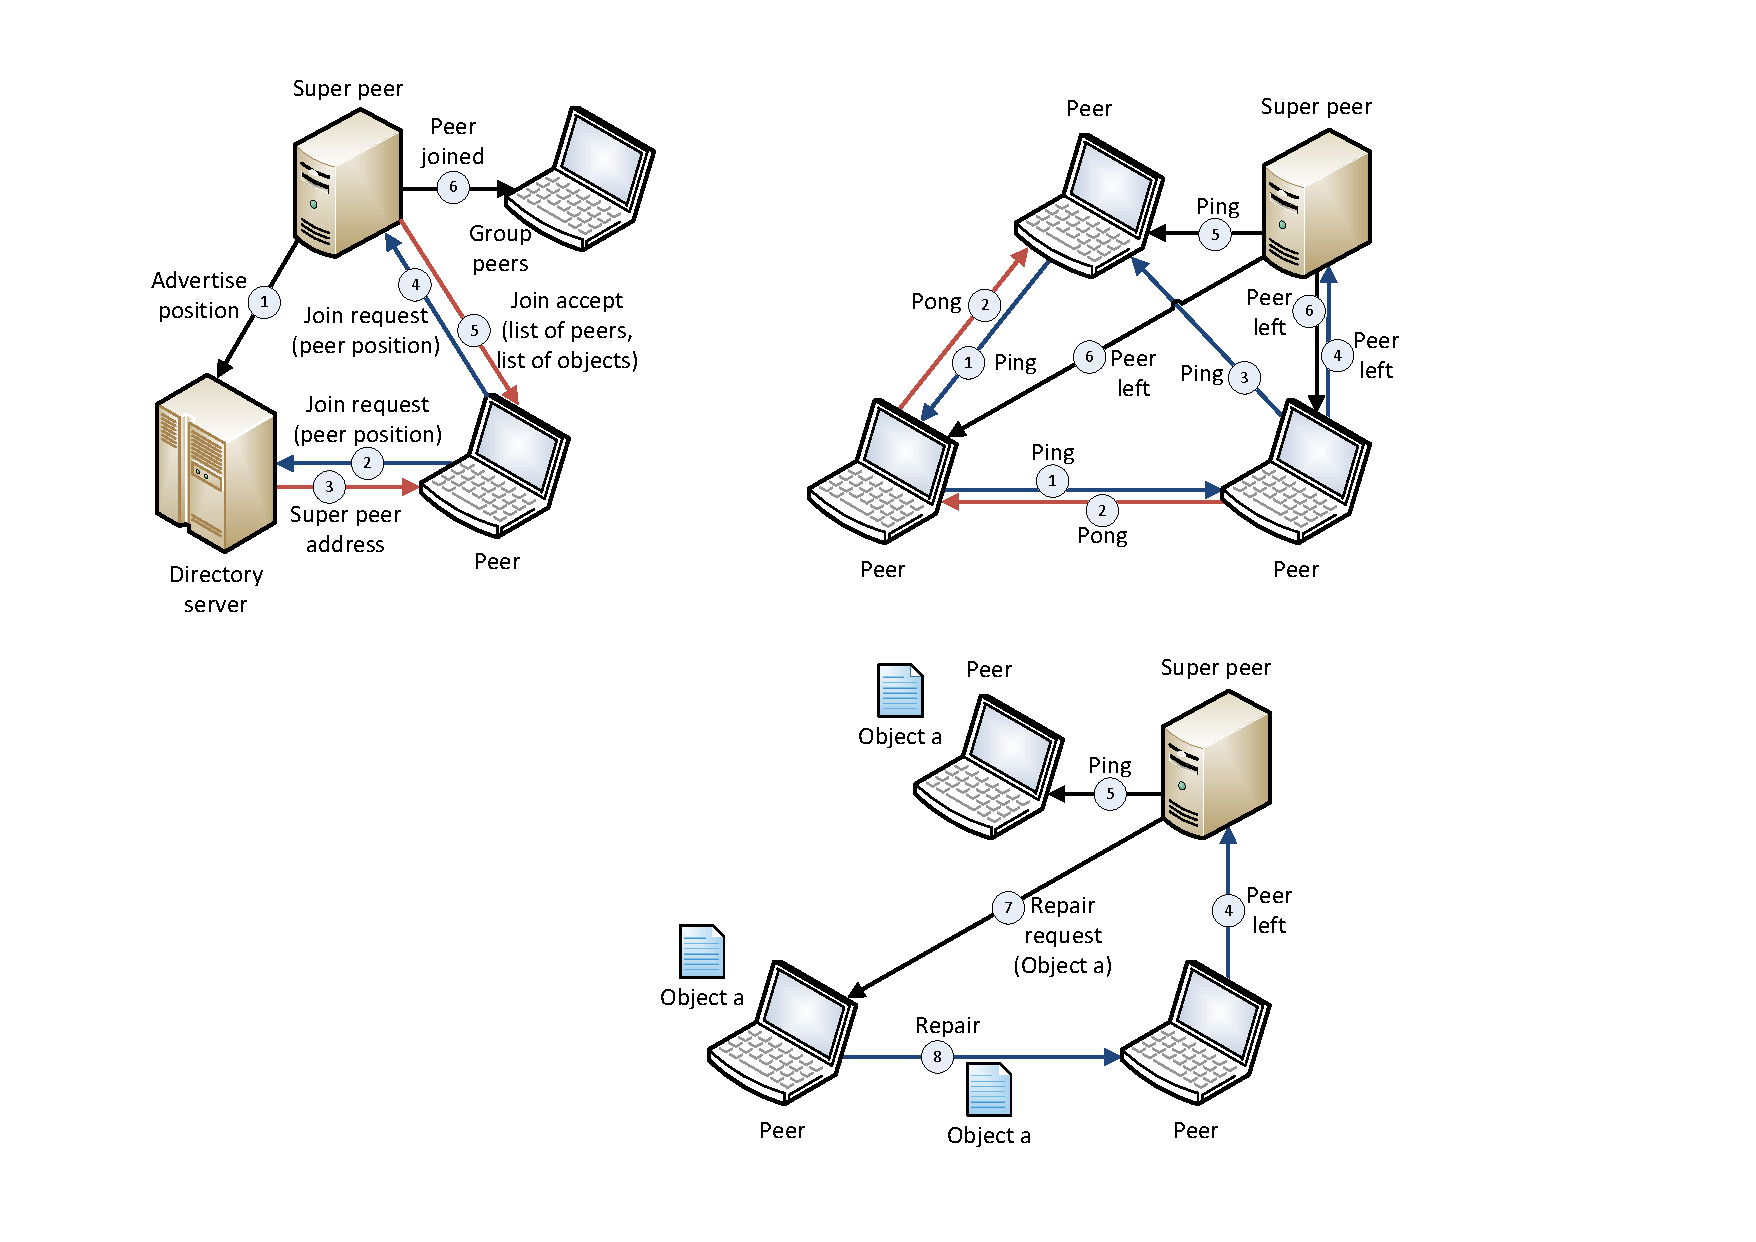
\includegraphics[clip=true, viewport=135mm 110mm 242mm 196mm, width=0.7\columnwidth]{Pithos_mechanisms}
 \caption{Pithos group leave mechanism. Two of the three peers respond to a ping request, while a single peer does not. That peer is removed from the group by the super peer.}
 \label{fig_pithos_leave}
\end{figure}

In Pithos, two methods exist to ensure group consistency and handle peers leaving the group. The first method, shown in Figure \ref{fig_pithos_leave}, uses periodic keep-alive messages as follows:
%
\begin{enumerate}
\item At regular intervals, each group peer uniformly randomly selects another peer in the group to send a keep-alive (Ping) message to.

\item If a peer received a keep-alive message, it responds with an acknowledge (Pong) message.

\item A peer that does not respond with an acknowledge message within a sufficiently large amount of time is considered to have left the network.

\item The originating peer of the keep alive message informs the super peer that the target of the keep-alive message is thought to have left the group.

\item The super peer then also sends a keep-alive message to the target peer, to ensure that there does not exist some communications issue between the two group peers, and that the target peer has actually left the network.

\item If the target peer does not respond to the super peer, the super peer informs all group peers that the target peer has left the group.
\end{enumerate}

The super peer verifies that the peer has left, because by design the super peer is selected to be the most available peer in the group on the network. The super peer does not transmit all keep-alive messages in order to prevent overloading of the super peer.

It is accepted that not all group peers might receive keep-alive messages every round, because of the random selection mechanisms, but this is not required. Only that in a sufficiently small number of keep-alive intervals, the peer is found to have left.

The second mechanism uses requests to identify peers that have left the group. Whenever a request is sent to another peer, a timeout is also started. If a peer does not respond to a request within a given amount of time, the same leave mechanism will be activated as if the target peer has not responded to a keep-alive message.

It should be noted that either of these methods are sufficient to ensure group consistency over some time period, but using both minimises the time it takes to detect a peer leaving the group.

For graceful group leaves, the same leave mechanisms as used in group migration is employed, which is to be discussed in the next section.

\subsubsection{Migration mechanism}
\label{migration_design}

Users will constantly be moving in the virtual environment, leading to changes in position. These position changes may lead to users moving from one group to another. It is imperative that all objects stored in Pithos remain available even with users traversing groups.

Group migration involves informing the group that the peer is leaving and initiating the group join mechanism. Informing the group that the peer is leaving ensures that this peer will not be picked for any storage or retrieval requests, while the group is unaware that the peer has left. If this is not done, the group will only know that a peer has left after a timeout for a request to the peer expires, which reduces request success rates.

There is a time window between a peer leaving a group and all peers being informed of the migration. During this time, a peer that has migrated might receive requests from its original group. The peer will serve these requests if able and include a group ID in its response. If a peer receives a response from another group, the requesting peer removes the responding peer from its group list. Inter-group requests are not currently allowed due to scalability concerns as time passes and peers continue to migrate.

The current implementation of the group migration mechanism is based on a centralised approach discussed in Section \ref{group_migration_implementation}.

\subsubsection{Ledgers and object store modules}

The previous sections have focussed on group storage, purely as an $O(1)$ structured overlay. To enable the storage and retrieval of objects within the group, an object store is also required, as well as a way to track which objects are stored on which peers and conversely, which peers contain which objects.

Each peer in the group contains a local authoritative object store, containing all objects stored on the peer by group storage. Each object is stored with an associated time-to-life (TTL) to prevent stale object copies.

Each peer and super peer in the network contain a group ledger to keep track of which objects are stored on which peers. The group ledger is required whenever an object is retrieved within the group to know from which peer an object can be requested. The ledger is also used by the super peer, to determine which objects should be repaired.

\subsubsection{Distance-based storage mechanism}
\label{distance_based_design}

For Pithos to succeed as an MMVE storage architecture, intra-group data requests should be preferred to inter-group data requests. This requirement, combined with the fact that the grouping algorithm geographically groups users in the virtual world, lends Pithos to a storage system based on distance-based storage. Similar to interest management, the assumption is that users have a limited area of interest and require interaction with a limited number of objects within range.

Distance-based storage is implemented on a group level rather than an individual level, which means that objects are stored on the nearest group of users, rather than the nearest user. It is assumed that such an approach will alleviate the security and reliability challenges present in distance-based storage \cite{gilmore_p2p_mmog_state_persistency}.

With group-based distance-based storage, it is assumed that because peers now store objects closest to the group, the objects that they are interested in will most likely be stored within their own group. Therefore, most data requests should be intra-group requests. The overlay storage component ensures that nodes that require data, which are not stored within their group, are still able to access requested data.

\subsection{Overlay storage (DHT) module}

The function of overlay storage is similar to that of group storage. It provides storage capabilities as a backup to group storage to improve reliability. Various overlay storage architectures exist, as discussed in Section \ref{overlay_storage}. Any existing overlay storage architecture can be used in Pithos.

The requirements of overlay storage is that is should be reliable, bandwidth efficient and able to handle network churn. It is assumed that a $O(\log(N))$ overlay is used. For the overlay storage, responsiveness is unimportant, since group storage ensures responsiveness. Reliability is the most important aspect of overlay storage.

An example of an overly storage that might be used in Pithos is PAST \cite{PAST_storage}, based on the Pastry overlay \cite{pastry}.

\subsection{Certification mechanism}

In order to design a secure distributed storage system, one requirement for the P2P overlay is that peers should not be able to select their own IDs or it will not be possible to secure the system against attack. Peer IDs should rather be assigned securely by some certification authority \cite{secure_overlay_routing}.

To meet this requirement, Pithos implements its own certification authority to assign peer IDs securely and promote security in the P2P overlay. A certification server exists that handle ID requests from peers. The server assigns IDs to peers and provides the peer with a signed certificate that it may use to store data.

Whenever an object is stored or updated in the storage network, peers have to sign the object to enable the tracking of object changes throughout the life of the object. This system is different from classic distributed file storage designs that advocate anonymity in storage. The fact that all changes can be tracked to a specific peer will simplify the task of eliminating user cheating.

\subsection{Quorum mechanism}
\label{quorum}

A security mechanism that performs object verification is also used. When this mechanism is activated, the objects received from multiple retrieve responses are compared to ensure object correctness.

Object verification is an attempt to make Pithos more resistant to malicious peers that attempt to alter data in a way that is not consistent with the environmental logic. When multiple retrieve responses are received, all objects are compared and the object that occurs the most from all the responses is sent to the higher layer.

\subsection{Replication mechanism}

When storing objects in Pithos, replication is used to increase object availability under network churn and for security in the presence of malicious peers \cite{storage_and_chaching_PAST}. For every object that is stored in Pithos, $R$ object replicas are also stored. The number of replicas ($R$) depends on the degree of network churn as well as the number of expected malicious users in the network. If the network churn is high, more replicas are required to avoid the situation where all $R$ peers hosting an object leaves the network before any object migration can be done.

If a peer leaves the network and stops to transmit ``keep alive'' messages, the repair mechanism will detect this and replicate the file on another peer. Replication exists on group as well as overlay storage and is required for ensuring that if a peers leaves the network, the objects that it stores are not lost.

In overlay storage, when the target of a retrieval request leaves the network, the request is routed to the peer with the next closest ID, because of the distance-based routing scheme used in overlay storage. This feature of overlay routing can be exploited by storing object replicas at peers with IDs that are close to the main peer selected to store the object. If a peer leaves the overlay, the new destination peers will possess the stored files, since overlay storage stores overlay replicas at overlay neighbours.

Group replication will be described in detail when the storage mechanism is described in Section \ref{pithos_store}.

Another reason to replicate objects is to make the system more secure. If it is known that a certain percentage of users are malicious, it is beneficial to have more replicas than malicious users. This will allow for a secure system where object hashes can be compared to determine which peers are malicious and what version of an object is accurate.

\subsection{Repair mechanism}

When objects are stored, as described in Section \ref{pithos_store}, multiple replicas of the same object is stored within a group. This form of redundancy extends the lifetime of an object, but with the presence of constant network churn, all objects will eventually cease to exist.

The solution is to use a repair mechanism to ensure that missing object replicas are constantly replaced. Two types of repair mechanisms were implemented: periodic repair and leaving repair.

With periodic repair, the super peer periodically checks the number of available replicas of every object in its group ledger. If an object contains less than the required number of replicas and there are peers in the group that do not already store the object, that object is replicated. Because the super peer itself contains no objects, it requests that an object be replicated from a peer that does contain the object. That peer will receive a repair request for a specific object, select a group peer in a uniformly random fashion, that does not already contain the object, and initiate a store request to that peer.

Object repair is not lossless. A peer can be selected to store a new object replica and that peer can leave the group before it stores the object. Because many object replicas exist and the loss of a single object will, therefore, not endanger the life of an object, the extra bandwidth and maintenance requirements could not be justified. Sometimes there are multiple object replicas missing, which is solved by having the super peer request multiple object repairs.

Since objects are only destroyed when a peer leaves the group, with leaving repair, the super peer repairs all objects of a peer that leaves the group. This mechanism can be seen as an extension of the group leave mechanism, depicted in Figure \ref{fig_pithos_leave}. Figure \ref{fig_pithos_repair} shows how this mechanisms is extended to include repair. Steps 1 to 6 are the same as for the leave mechanism.

\begin{figure}[htbp]
 \centering
 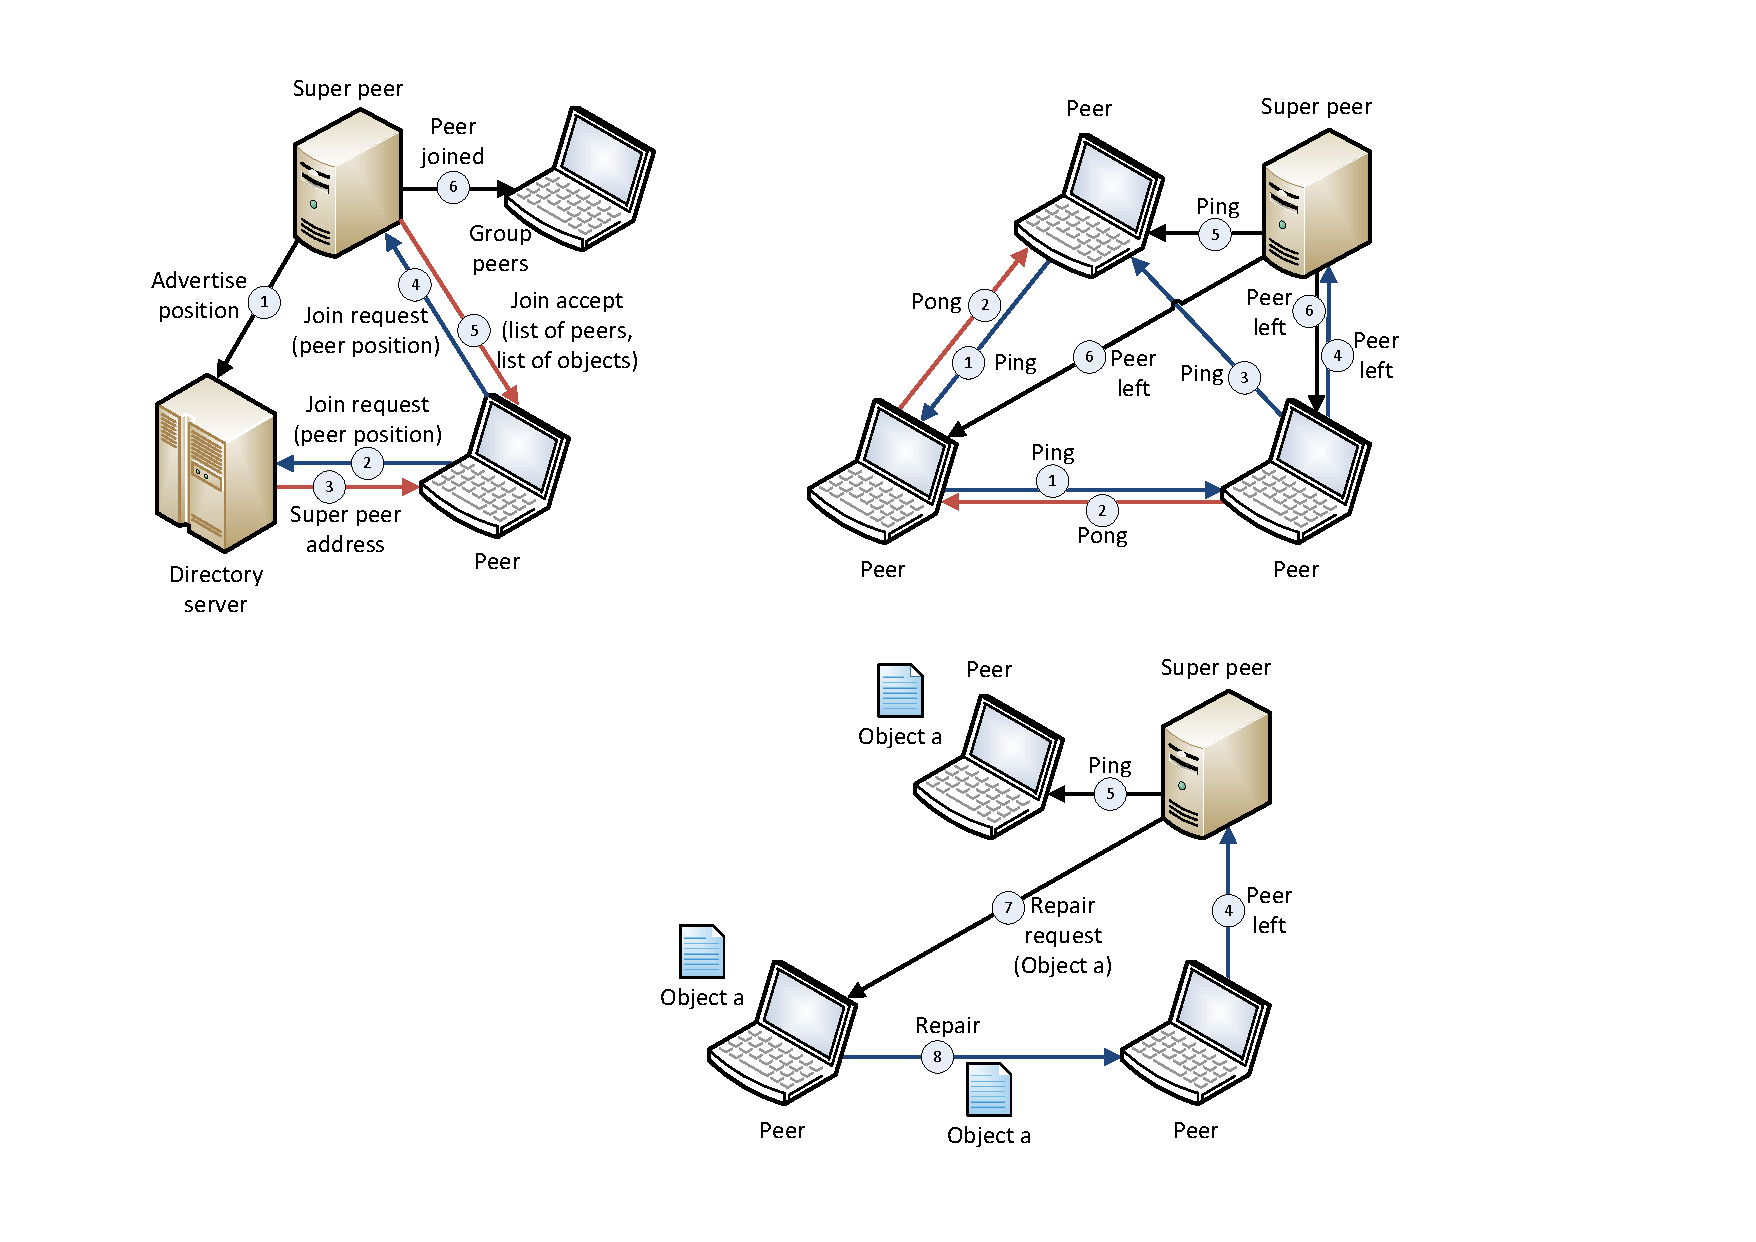
\includegraphics[clip=true, viewport=110mm 15mm 225mm 100mm, width=0.7\columnwidth]{Pithos_mechanisms}
 \caption{Pithos repair mechanism. The super peer requests that Object a be replicated on the only peer in the group that does not yet store it.}
 \label{fig_pithos_repair}
\end{figure}
%
\begin{enumerate}
\setcounter{enumi}{6}
\item After a the super peer has detected that a peer has left and has informed all other peers, the super peer selects a peer that contains an object that was destroyed by the leaving peer and requests that that object be replicated.

\item The peer receiving the replication request from the super peer selects another peer in the group that does not already contain the object and replicates the object on the selected peer.
\end{enumerate}

Leaving repair attempts to minimise the super peer load by only repairing objects when a node leaves the network. This is as opposed to periodic repair, where the super peer has to constantly cycle though its list of object replicas and verify the number of replicas currently stored in the system.

\section{Satisfying the use cases}
All Pithos modules and mechanisms that ensure adherence to the storage requirements have now been described. What remains to be described is how the use cases presented in Section \ref{use_cases_goals} are designed on the architecture that adheres to the storage requirements.

It is assumed that some higher layer exists above Pithos, which generates requests. According to our generic consistency model, these requests will arrive from the environment logic or object updater. It should be noted that a request can be a storage, retrieval, modification or removal request and does not only imply a request for data, i.e. a retrieval request.

\subsection{Store}
\label{pithos_store}

\begin{figure}[htbp]
 \centering
 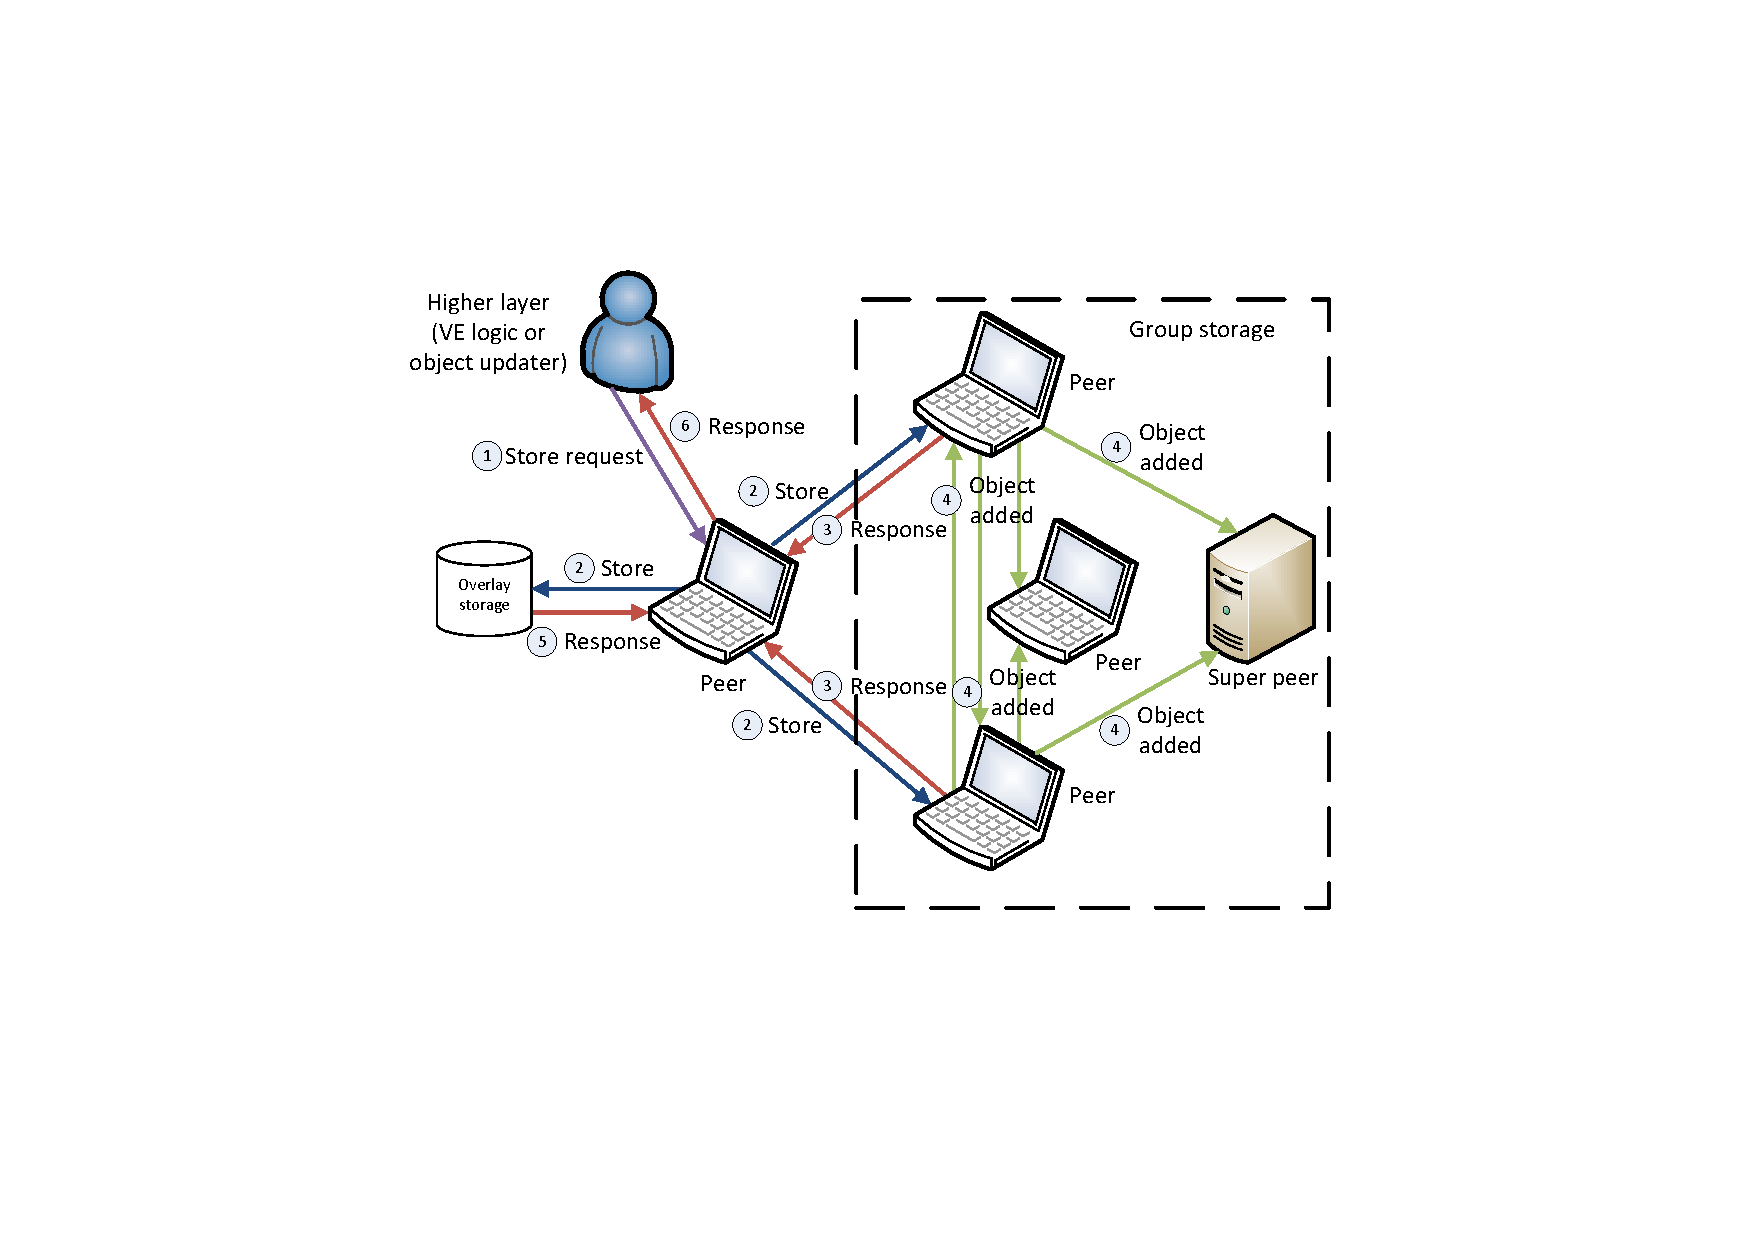
\includegraphics[clip=true, viewport=67mm 55mm 228mm 165mm, width=0.7\columnwidth]{Pithos_use_case_store}
 \caption{Pithos storage. The higher layer requests that an object be stored. The peer stores the object both in overlay storage and group storage.}
 \label{fig_pithos_storage}
\end{figure}
%
Referring to Figure \ref{fig_pithos_storage}, Pithos storage works as follows:
%
\begin{enumerate}
\item The higher layer is expected to send a storage request to the Pithos module on the source node, containing the object to be stored.

\item Pithos contains logic that relays the storage request to peers in both group storage and overlay storage.

\item The group storage module will store the object in its local authoritative object store and acknowledge the reception of the object by sending a response message to the source node.

\item Each peer successfully storing a received object will inform all group peers, as well as the super peer, of the new object stored. The peers and super peer can add this information to their group ledger, used to service retrieval requests.

\item Overlay storage also completes the request and informs the source node of the success or failure of the request, by sending a response message.

\item The Pithos module on the source node monitors all responses and records the success or failure of each request. When a sufficient number of responses have been recorded, Pithos informs the higher layer of either a successful or failed store.
\end{enumerate}

Overlay storage implements an existing DHT and it is assumed that overlay storage correctly handles the storage request.

The number of nodes selected from the group ledger for storage relates to the number of required object replicas. Nodes are selected in a uniformly random fashion, making sure to never select the same node more than once. If a node is selected more than once, it reduces the effective number of replicas in the network, which reduces the expected object lifetime. \footnote{A detailed discussion of object lifetime is presented in Chapter \ref{chp:MODELLING}.}

The question arises as to what constitutes a sufficient number of responses. Two types of storage mechanisms have been implemented in Pithos: ``safe'' and ``fast''. When safe storage is used, Pithos waits for all responses to be received. Only after all responses are received is a decision made whether the store was successful or not. If the majority of group stores as well as the overlay store are successful, is the request considered to be a successful store. The higher layer is then informed of the status of the store request.

When fast storage is used, Pithos only waits for the first successful response, before informing the higher layer of success. Only if all responses are failures is the higher layer informed of a failure.

Because safe storage ensures that most of the replications are successfully stored, there is a smaller chance of it reporting a false positive than for fast storage. The disadvantage is that from the point of view of the higher layer, and by extension any system that uses Pithos, safe storage requests have a lower responsiveness. Fast storage on the other hand is no less reliable than safe storage, but the chances of a false positive being reported to the higher layer is greater. The advantage of fast storage is that the from the perspective of the module using Pithos, it is performed faster than safe storage. A comparison of fast and safe storage is performed in Chapter \ref{chp:EVALUATION}.

\subsection{Retrieve}
\label{pithos_retrieve}

%Talk about the types of keys (content key and name key) and how objects will be named in the storage system.

\begin{figure}[htbp]
 \centering
 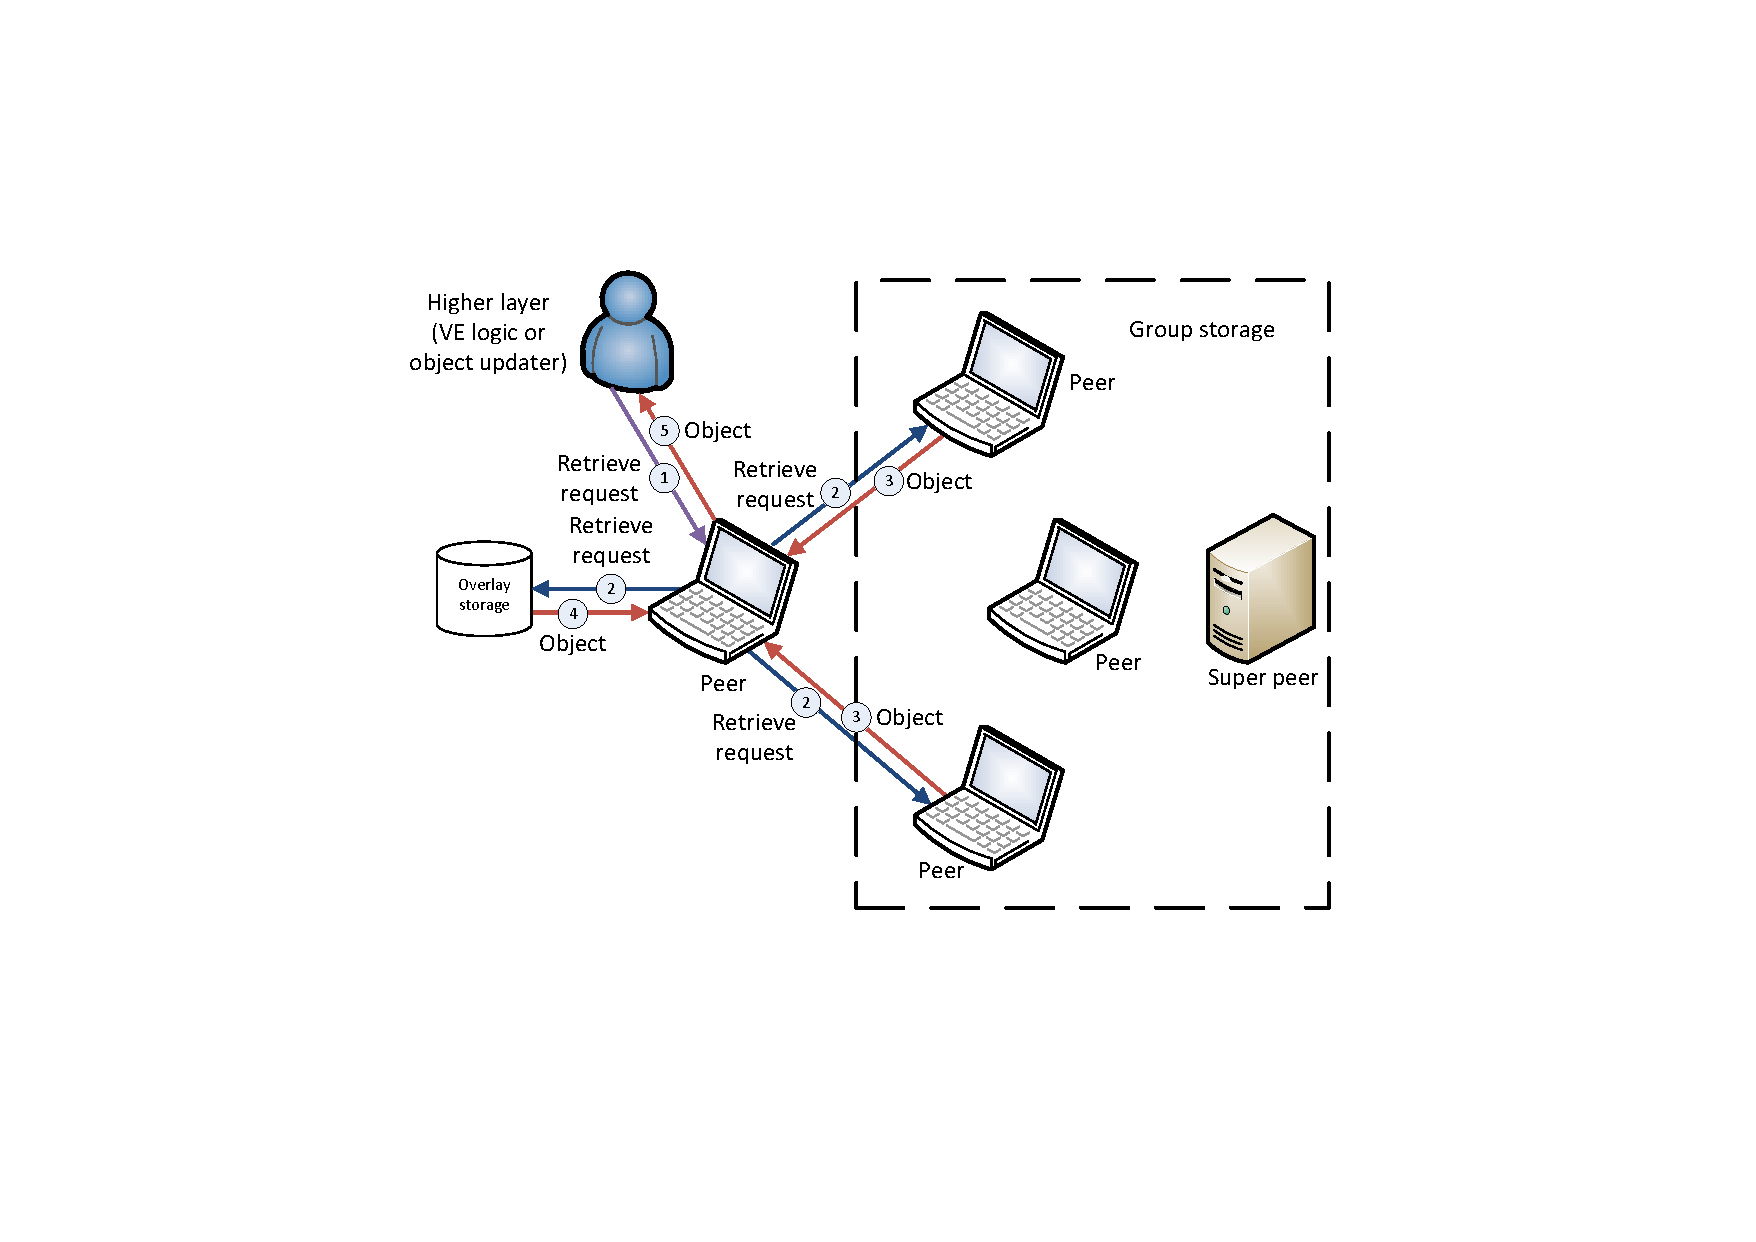
\includegraphics[clip=true, viewport=67mm 55mm 228mm 165mm, width=0.7\columnwidth]{Pithos_use_case_retrieve}
 \caption{Pithos retrieval. The higher layer requests that an object be retrieved. The peer requests the object both from overlay storage and group storage.}
 \label{fig_pithos_retrieval}
\end{figure}
%
The process of retrieving object data is similar to that of storing object data. With reference to Figure \ref{fig_pithos_retrieval}, retrieval works as follows:
%
\begin{enumerate}
\item The retrieve request, received from the higher layer, contains the hash of the object name which the higher layer requires.

\item Pithos first checks whether the object that was requested exists within the group by checking its group ledger. This is required, because the higher layer might have requested an object that is stored in another group. Out-of-group requests are only serviced by overlay storage. If the object is housed in the Pithos peer's local store, the object is sent to the higher layer. If the object is not housed locally, Pithos requests the object from both overlay and group storage.

    The group ledger is used to determine which group peers contain which objects. The number of peers selected depends on the retrieval type. Three retrieval types exist: fast, parallel and safe retrieval. Fast retrieval selects a single peer for object retrieval. Parallel and safe retrieval select multiple peers to concurrently retrieve an object from. More requests sent in parallel improves the probability of the request succeeding as well as reducing the time it takes to serve the request.

\item When the retrieval request is received at the destination peer, the object is retrieved from local storage, attached to a response message and sent to the requesting peer.

\item Sometime after group retrieval has completed, overlay retrieval will also complete and send the object, stored in the overlay, to Pithos.

\item After Pithos has received a sufficient number of responses, it informs the higher layer of either a successful or failed retrieval. The object itself is attached to a successful request response.
\end{enumerate}

Retrieve requests mainly fail because of nodes leaving a group. If a node leaves before it can serve an object, the object request fails. If multiple requests are sent with parallel retrieval, it improves the chances of contacting a node that is not about to leave, which improves the probability of retrieval success. More requests also improve lookup times, since some peers might be geographically closer to the requesting peer, thereby possessing a lower latency.

Sending multiple requests improves the chances of contacting a peer that is closer, which improves the responsiveness of the systems. Fast and parallel retrieval sends the first successful  response, and therefore, the first successful object, to the higher layer. It replies with failure if all requests failed. The disadvantage is that it is not resistant to malicious peers.

The safe retrieval request is more resistent to malicious nodes. For safe retrieval, Pithos waits for a specified number of responses in order to use the quorum mechanism described in Section \ref{quorum}.

As shown in Figure \ref{fig_pithos_retrieval}, the super peer is not used for retrieval requests. This is not necessary, since all peers contain lists of all objects. The super peer should, however, still contain its own group ledger, to inform peers joining the group of the peers and objects already in the group. Not requiring the super peer to manage object requests prevents the super peer from becoming overloaded.

\subsection{Modify}

Modifying data is similar to storing data. A request to modify a specific object is received from the higher layer. The request specifies the object ID, the parameter that has to be modified and the new value of the parameter. The update is delivered to Pithos, which forwards the request to both group and overlay storage. The overlay handles the modify request and responds with success or failure. Group storage received the modify request and checks the group ledger whether the object exists within the group. If the object does not exist in the group, it is only modified in the overlay. To keep track of modified objects, each object has a version number that is incremented every time an object is modified. This allows retrieve requests to select the object with the latest version number to be sent to the higher layer.

If the object exists within the group, all peers that contain the object are identified from the group ledger and modify requests are sent to them. The modify request is sent to the destination peer, where the object in the local store is updated and its version number incremented. If a retrieve request receives objects with multiple version numbers, it selects the set of objects with the latest version number for ``safe'' comparison.

\subsection{Remove}
\label{remove_use_case}

Removal is handled by the object TTL. It is not possible to define an explicit remove operation for overlay storage, since a peer may be off-line when the removal request is sent. If the peer rejoins the network, the object becomes available again. Object TTL ensures that the storage space requirements does not increase indefinitely during the lifetime of the storage system.

\section{Conclusion}

This section describes the Pithos conceptual design. Pithos is a hierarchical distributed storage system that uses grouping to reduce latencies of store and retrieve requests, as is required by massively multi-user virtual environments (MMVEs). The use cases are defined from the perspective of the higher layer that wishes to make use of Pithos's services.

The conceptual design is first described in terms of how it ensures the storage requirements are met. Each module and mechanism that contributes to the achievement of the identified requirements are then discussed. The implementation of the use cases is described with a discussion of how they relate to the modules and mechanisms required to ensure the consistency requirements are met.

Pithos is designed as a multi-tiered distributed storage system, containing multiple $O(1)$ group stores and a single $O(\log(N)$ overlay store. Each node is connected to the overlay storage and grouped into group storage. A certification mechanisms ensures store and retrieve requests can be tracked and that malicious users can be identified. It contains a quorum mechanism that rejects maliciously altered objects. To maintain reliability, a replication redundance mechanism with repair is used.

Group storage has a fully connected network topology, containing peers and super peers. Ledgers allow each peer in a group to keep track of all other group peers and all objects available on the group peers. Distance-based storage is used to ensure that retrieval requests for objects in the VE are mostly within the same group.

Every storage, retrieval and modification request is sent to both overlay and group storage. Group storage makes use of the group ledgers to find object locations for retrieval and possible peers for storage. Removal is ensured by the association of a TTL with all objects.
